\documentclass{article} % For LaTeX2e
\usepackage{nips15submit_e,times}
\usepackage{hyperref}
\usepackage{url}
\usepackage{pdfpages}
\usepackage{float}
%\documentstyle[nips14submit_09,times,art10]{article} % For LaTeX 2.09


\title{SakaiAtMidnight 521 Final Project}


\author{
  Leonardo Shu\\
  Department of Statistics\\
  Duke University\\
  \texttt{leonardo.shu@duke.edu} \\
  \And
  Mengrun Li \\
  Department of Statistics\\
  Duke University\\
  \texttt{mengrun.li@duke.edu} \\
  \AND
  Yaqian Cheng \\
  Department of Statistics\\
  Duke University\\
  \texttt{yaqian.cheng@duke.edu} \\
  \And
  Wei (Emily) Shao \\
  Department of Statistics\\
  Duke University\\
  \texttt{wei.shao@duke.edu} \\
}


\newcommand{\fix}{\marginpar{FIX}}
\newcommand{\new}{\marginpar{NEW}}

\nipsfinalcopy % Uncomment for camera-ready version

\begin{document}


\maketitle

\begin{abstract}
This project attempts to choose the best type of logistic regression model to predict the results of the 2012-2015 NCAA tournaments using detailed regular season data for all the teams in the association.
\end{abstract}

\section{Introduction}

The goal of our final project is to predict results of various NCAA tournaments with a variety of models and compare the results to figure out which one, if any, works best. This is a quite popular excercise done every year during March Madness but there is still a lot of debate as to the best method of prediction apart from blind guessing and being biased for one's favourite team. A few papers have been written about this sort of problem. In \textit{Bracketology: How can math help?}[1], the authors predict brackets by calculating ratings of each team using linear systems of equations.

The data sets we will be using are provided by a past competition on Kaggle.com, which ensures that we are using information which is both reliable and rich enough for our project goals. The data sets have detailed information on past NCAA regular seasons, tournaments, along with seeds and ID's for each team to facilitate prediction match-ups. Specifically, there are more than 5000 pieces of game data for each year, including 34 columns of relevant game statstics for each playing team such as field goals made, number of blocks, number of steals and number of assists, which will be essential for us to measure a team's performance.

Since we already know the resulting "true" brackets of past tournaments, we can easily rate how our predictions did with a complete set of results. However, since the odds of predicting a bracket is theoretically 1 in 9.2 quintillion[2] and even betting sites or fan competitions never exactly search for "perfect" brackets, we did not want to assess our predictions solely on perfection either. As a result, we are going to divide our predictions into different levels of accuracy where we see how our model performs in predicting each round of the tournament, from the Second Round (post First Four) to the Championship game.

\section{Methodology}
\label{gen_inst}

\subsection{Model Setup / Data Manipulation}
All of our four models are going to be a variation of logistic regression. We are going to compare predictions between LASSO, Ridge, Elastic Net and Bayesian GLM with stepwise method. With the last method after we get coefficient estimates from Bayesian GLM, we use stepwise to select significant coefficients. The Bayesian model assumes an independent normal prior for each coefficient and performs MCMC algorithm to search for posterior of each coeffiecient. Then we select the most significant coefficients calculated by Bayesian GLM using stepwise method from both directions.\
Each model will be trained at first by using data from the regular season of that tournament's year. Afterwards, each game in that tournament will be predicted by using the average seasonal performance of both teams. Since for every tournament we already know the starting 32 games and all seeds in every region, we can predict each game's result from the second round and use our model to progressively fill in the whole tournament bracket, we then evaluate our model's performance by seeing how it matches the true events.

We start out with our full logistic model $Y_{ab} = X_{ab}^T \beta$ where:\
\[ Y_{ab} = \left\{
\begin{array}{ll}
1 & Team \ a \ wins \\
0 &  Team \ b \ wins \\
\end{array} 
\right. \]\
$X_{ab}$ is a matrix of all 32 relevant statistics for teams a and b, with each row indicating one game in the regular season of the year in question. Finally, $\beta$ is a vector of the corresponding coefficients for each column of $X_{ab}$.\ One of the main differences between each model will stem from the way they perform variable selection, affecting the size of $X_{ab}$.\\

An early challenge we faced was to figure out what amount of regular season data we use to train our models. At first it seems that more data always helps, especially from an immediate previous season, to describe average team capabilities.  However, we can also argue that it doesn't make sense to use data from seasons too far back from the tournament we want to predict since there is a huge turnover in players and strategies, even if coaches and philosophies remain.

To answer this issue, we ran each model to predict the 2015 tournament with data from the 2015, 2014 and 2013 seasons. The resulting plots can be seen in Figure 1 of the Appendix. Across all four models there is clear improvement in prediction rates per round when 2-year data is used but not 3-year data. Notably, the LASSO and Elastic Net models benefit the most of regular season game information. Thus, from our prediction models will always be trained with data from the past 2 seasons of that tournament's year.

\subsection{Coefficient Analysis}

In our four models, LASSO, Elastic Net and Bayes GLM can do covariates selection. Checking the non-zero coefficients of the results, we can see some surprising results. First of all, the coefficients for each team are either significant or not in pairs. Which means that there is no case where assists for team a are important but assists for team b are not. Second, the final scores for each team at the end of each game are not relevant enough to be used which is quite unintuitive since these numbers logically determine the winner of the game. But with this result, we do not have to worry that such a statistic would cause overfitting issues to our model.\

Although the covariates selection may be slightly different when we add data of previous years, in general, they choose almost the same predictors. The coefficients of different predictors selected with different years data are very insignificant. That means they do not contribute too much to our model.\

\section{Results / Predictions}

The results we obtained from our various models are split across Tables 2-5 in the Appendix categorized by each year from 2012-2015, with the prediction rate for each model (i.e the percentage of total games correctly predicted) at each round listed. We note that each percentage must be viewed with careful consideration. For example, a low value in the Final Four does not immediately imply a bad predicted bracket since the number of winners to be predicted (4) is much less than in the second round (32) so this does not mean our predictions for the subsequent rounds are without value.

\subsection{Second Round: 32 games}

Throughout the four tournament editions, our models' predictions for this round were the highest of them all, but this is unsurprising since predictions of the following rounds depend heavily on whether the prediction made are correct or not (E.g Predicting two consecutive games unsuccessfully, automatically makes the prediction for the game between those "incorrect" winners wrong). However, we stil get respectable ranges of 0.6 to about 0.9 accuracy. Historically, no No.1 seed has ever been upset by a No.16 seed in NCAA history so we know that in this round at least, the seeds ranking are very good predictors. Our model favours stronger seeds by construction so it will have high prediction rates. The results for each model are also notably consistent. We can rank our models from worst to best in the following order: LASSO $<$ Elastic Net $<$ Bayes GLM $<$ Ridge.

\subsection{Third Round: 16 games}

The Third round is overall proved to be a much harder round to predict. All of our models have rates between 0.1 to 0.6 which is alot of variation for a single round unlike before. Here we can see first-hand the difficulties our models encounter when upsets are not considered to a large extent. Most of our mispredictions come from these type of games and even one or two upsets can go on to shatter future predictions. Even so we can still rank our models' perofrmance: Bayes GLM $<$ Ridge $<$ Elastic Net $<$ Lasso.

\subsection{Sweet Sixteen: 8 games}

This round has quite regular patterns in prediction rates for all four tournaments despite the lower values (0.1 to 0.3) and since the number of games is halved, this unfortunately means the overall predictions are worse than before. However, this should not come as a surprise because at this stage of the brackets the seeds of the teams start to lose some of their meaning as usually most of the strongest remain so the skills start to converge such that clear favourites are less apparent. The model ranks are change considerably from before: Lasso  $<$ Elastic Net $<$ Bayes GLM $<$ Ridge.   

\subsection{Elite Eight: 4 games}

At a close glance, the most common rate in this round is 0.25. On one hand, we can take some confidence in that our model can regularly predict some true results at this deep stage of the tournament. On the other hand, only predicting one winner drastically lowers the chances of getting decent rates for the final two rounds. That being said, the Ridge model did manage to get 0.5 and 0.75 rates in 2012 and 2015 respectively. This were our best estimates and a great example of how a bracket can still be "fixed" even if many games were mispredicted. In these particular cases, most of the No.1 seeds from each region made it to the Final Four. Since, our model naturally favours those teams with better seasonal performances (the teams that become the strongest seeds), these predictions are not anomalies. Model ranks: Lasso  $<$ Elastic Net $<$ Bayes GLM $<$ Ridge.  

\subsection{Semi-Finals: 2 games}

Here we curiously get the same rates across all models and only in 2012 and 2013 do we get a 0.5 rate (1 game), otherwise the rest of the years get 0 rates. Again, this isn't a failure but rather points out to where improvements can be made to our models. At this point of the tournament, we have the four strongest teams of the conference and only very rarely will most of them be unexpected upset teams. More than likely, the teams will be similarly skilled colleges and our models will have a hard time predicting the winner when the margins between teams are not very significant. Model Ranks for Semis: Lasso  = Elastic Net = Bayes GLM = Ridge.  

\subsection{Championship Final: 1 game}
Given that the previous round has almost always has incredibly low prediction rates, determining the champion will be very unlikely. In fact, none of our models could do it but we can't say our models have failed to be useful. Model Ranks for Final: NA

\subsection{Best Model}

All four models analyzed appear to have different levels of precision per round of the tournament. Interestingly, we see that the LASSO and Elastic Net have quite similar performances, the same applies between Ridge and Bayes GLM. Yet as we look at the prediction rates of the tournaments we used, the logistic Ridge regression model was constantly one of the better predictors at every stage. Multiple reasons might explain this: The Ridge penalty could be the best tuning parameter for NCAA game data. Unlike the other models which ignore many contents of the data, the Ridge model uses all the covariates provided. Not only will the fit be better, but the statistics such as team scores, blocks and steals made that intuitively should affect game outcomes are taken into consideration for the predictions.

Our best bracket was for the 2015 tournament (coincidentially, our initial main goal to predict) using Ridge regression and can be seen in Figure 1 of the appendix. We can attribute this result to the fact that the latter rounds did not experience a lot of upsets and most of the No.1 seeds made it to the Final Four. These situations benefit our model specifications greatly as we mostly value the teams with the highest consistency all year long.\

\section{Model Improvements: Account for Upsets}

To account for upsets that our model has not explained, we examine the history of every paired game in the 2015 bracket and record the information whether they have played in regular seasons between 2003 and 2014. Since in tournament most of times two teams from different regions did not play against each other in regular seasons, out of 67 games, only 19 games have happened in regular seasons during the past 12 years. For every paired game in the bracket, we use the following formula to compute proportion of strong seed A beat weak seed B conditional on only games of strong seed A played against weak seed B in the past:

$P=\frac{Number \ of \ times \ strong \ seed \ A \ won \ - \ Number \ of \ times \ weak \ seed \ B \ won}{Number \ of \ times \ strong \ seed \ A \ played \ against \ weak \ seed \ B }$


The results are shown in the table below. In 14 out of 19 games historical records indicate consistency with actual tournament results. One of the historical records somewhat explains an upset game in our model prediction when the data shows Villanova were beat by NC State in 2008 which is consistent with the actual tournament results, while our model predicts Villanova to win and show up in the final four. 

This further suggests that if we want to incorporate team specifics into our model to make our model more accurate, in each step after we apply the model to select two teams to play in the bracket, we would investigate the regular season information to determine whether strong seed A will beat weak seed B. However, since past information does not always inform future, we could possibily assign weights to teams in our regression model to consider possibility of an upset that may happen. 


% latex table generated in R 3.2.2 by xtable 1.8-0 package
% Mon Nov 23 16:47:50 2015
\begin{table}[ht]
\centering
\begin{tabular}{rrrrrrrrr}
\hline
& W & W3L1 & W1L2 & W1L1 & L & Correct & Games played & Correct proportion \\ 
\hline
& 9.00 & 1.00 & 1.00 & 2.00 & 6.00 & 14.00 & 19.00 & 0.74 \\ 
\hline
\end{tabular}

\caption{W: number of times strong seed A always beat weak seed B; W3L1: number of times strong seed A won three times as it was beat by weak seed B; W1L2: number of times strong seed A was beat by weak seed B as twice as it beat weak seed B; W1L1: number of times strong seed A won as many times as it was beat by weak seed B; Correct: Historical results indicates consistency with actual tournament results; Games played: number of games played; Correct Proportion: proportion that historical results indicates consistency with actual tournament results}
\end{table}





\section{References $\&$ Data Links}
[1] Chartier, Tim., Kreutzer, Erich., Langville,  Amy. and Pedings, Kathryn. Bracketology: How can math help? URL http://mathaware.org/mam/2010/essays/ChartierBracketology.pdf

[2] http://www.businessinsider.com/odds-of-perfect-ncaa-bracket-2015-3

[3] https://www.kaggle.com/c/march-machine-learning-mania-2015






\section{Appendix}
\begin{table}[H]
\centering
{\small
\begin{tabular}{rrrrr}
  \hline
 & LASSO & Elastic Net & Ridge & Bayesglm \\ 
  \hline
(Intercept) & -0.403 & -0.614 & -0.166 & -2.737 \\ 
  a.score & - & - & -0.023 & - \\ 
  b.score & - & - & 0.046 & - \\ 
  numot & -0.040 & -0.112 & -0.086 & - \\ 
  a.fgm & 6.223 & 9.809 & 1.182 & 42.818 \\ 
  a.fga & - & - & -0.071 & - \\ 
  a.fgm3 & 1.788 & 3.082 & 0.573 & 13.109 \\ 
  a.fga3 & - & -0.078 & -0.167 & - \\ 
  a.ftm & 4.051 & 6.189 & 0.677 & 28.922 \\ 
  a.fta & 0.164 & 0.453 & 0.374 & - \\ 
  a.or & - & -0.078 & -0.148 & - \\ 
  a.dr & 0.004 & 0.328 & 0.506 & - \\ 
  a.ast & 0.087 & 0.192 & 0.414 & - \\ 
  a.to & -0.035 & -0.301 & -0.380 & - \\ 
  a.stl & - & 0.025 & 0.169 & - \\ 
  a.blk & 0.021 & 0.090 & 0.184 & - \\ 
  a.pf & - & -0.040 & -0.304 & - \\ 
  b.fgm & -6.185 & -9.748 & -1.161 & -42.606 \\ 
  b.fga & 0.058 & 0.138 & 0.140 & - \\ 
  b.fgm3 & -1.773 & -3.140 & -0.622 & -12.807 \\ 
  b.fga3 & - & 0.188 & 0.233 & - \\ 
  b.ftm & -4.022 & -6.160 & -0.667 & -28.566 \\ 
  b.fta & -0.311 & -0.588 & -0.431 & - \\ 
  b.or & - & - & 0.084 & - \\ 
  b.dr & - & -0.156 & -0.493 & - \\ 
  b.ast & -0.023 & -0.126 & -0.404 & - \\ 
  b.to & - & 0.269 & 0.347 & - \\ 
  b.stl & - & -0.060 & -0.144 & - \\ 
  b.blk & - & -0.058 & -0.086 & - \\ 
  b.pf & 0.196 & 0.286 & 0.389 & - \\ 
   \hline
\end{tabular}
}
\caption{Coefficients estimates for 2015}\
\end{table}
\begin{table}[H]
\centering
{\small
\begin{tabular}{rrrrr}
  \hline
 Notation & Meaning \\ 
  \hline
  score & number of times scored \\
  numot & number of overtime periods \\
  fgm  & field goals made \\ 
  fga  & field goals attempted \\ 
  fgm3 &  three pointers made \\ 
  fga3 &  three pointers attempted \\ 
  ftm &  free throws made \\ 
  fta &  free throws attempted \\
  or & offensive rebounds \\
  dr & defensive rebounds \\
  ast & assists \\
  to & turnovers \\
  stl &  steals \\
  blk & blocks \\
  pf & personal fouls \\
   \hline
\end{tabular}
}
\caption{Notation explanation. "a." at front means team a; "b." at front means team b} 
\end{table}
\begin{table}[H]
\centering
{\small
\begin{tabular}{rrrrr}
  \hline
 & LASSO & Elastic Net & Ridge & Bayesglm \\ 
  \hline
Second Round & 0.594 & 0.625 & 0.531 & 0.625 \\ 
  Third Round & 0.438 & 0.375 & 0.312 & 0.188 \\ 
  Sweet 16 & 0.250 & 0.250 & 0.250 & 0.375 \\ 
  Elite 8 & 0.250 & 0.250 & 0.250 & 0.250 \\ 
  Simi-Final & 0.500 & 0.500 & 0.500 & 0.500 \\ 
  Final & 0.000 & 0.000 & 0.000 & 0.000 \\ 
   \hline
\end{tabular}
}
\caption{Prediction rate for each round in 2012}\ 

\centering
{\small
\begin{tabular}{rrrrr}
  \hline
 & LASSO & Elastic Net & Ridge & Bayesglm \\ 
  \hline
Second Round & 0.750 & 0.688 & 0.688 & 0.688 \\ 
  Third Round & 0.375 & 0.250 & 0.250 & 0.250 \\ 
  Sweet 16 & 0.250 & 0.125 & 0.125 & 0.125 \\ 
  Elite 8 & 0.250 & 0.250 & 0.250 & 0.250 \\ 
  Simi-Final & 0.500 & 0.500 & 0.500 & 0.500 \\ 
  Final & 0.000 & 0.000 & 0.000 & 0.000 \\ 
   \hline
\end{tabular}
}
\caption{Prediction rate for each round in 2013}\ 

\centering
{\small
\begin{tabular}{rrrrr}
  \hline
 & LASSO & Elastic Net & Ridge & Bayesglm \\ 
  \hline
Second Round & 0.688 & 0.656 & 0.594 & 0.750 \\ 
  Third Round & 0.312 & 0.125 & 0.188 & 0.375 \\ 
  Sweet 16 & 0.125 & 0.250 & 0.125 & 0.250 \\ 
  Elite 8 & 0.000 & 0.250 & 0.000 & 0.250 \\ 
  Simi-Final & 0.000 & 0.000 & 0.000 & 0.000 \\ 
  Final & 0.000 & 0.000 & 0.000 & 0.000 \\ 
   \hline
\end{tabular}
}
\caption{Prediction rate for each round in 2014}\ 

\centering
{\small
\begin{tabular}{rrrrr}
  \hline
 & LASSO & Elastic Net & Ridge & Bayesglm \\ 
  \hline
Second Round & 0.844 & 0.844 & 0.875 & 0.875 \\ 
  Third Round & 0.562 & 0.625 & 0.500 & 0.500 \\ 
  Sweet 16 & 0.375 & 0.375 & 0.375 & 0.375 \\ 
  Elite 8 & 0.500 & 0.500 & 0.750 & 0.750 \\ 
  Simi-Final & 0.000 & 0.000 & 0.000 & 0.000 \\ 
  Final & 0.000 & 0.000 & 0.000 & 0.000 \\ 
   \hline
\end{tabular}
}
\caption{Prediction rate for each round in 2015}\

\centering
{\small
\begin{tabular}{rrrrr}
  \hline
 & LASSO & Elastic Net & Ridge & Bayesglm \\ 
  \hline
Second Round & 0.84 & 0.84 & 0.88 & 0.88 \\ 
  Third Round & 0.56 & 0.62 & 0.50 & 0.50 \\ 
  Sweet 16 & 0.38 & 0.38 & 0.38 & 0.38 \\ 
  Elite 8 & 0.50 & 0.50 & 0.75 & 0.75 \\ 
  Semi-Final & 0.00 & 0.00 & 0.00 & 0.00 \\ 
  Final & 0.00 & 0.00 & 0.00 & 0.00 \\ 
   \hline
\end{tabular}
}
\caption{Prediction rate for each round in 2015 using regular season data from 2014-2015}\ 

\centering
{\small
\begin{tabular}{rrrrr}
  \hline
 & LASSO & Elastic Net & Ridge & Bayesglm \\ 
  \hline
Second Round & 0.84 & 0.84 & 0.84 & 0.84 \\ 
  Third Round & 0.38 & 0.38 & 0.50 & 0.56 \\ 
  Sweet 16 & 0.25 & 0.25 & 0.38 & 0.38 \\ 
  Elite 8 & 0.50 & 0.50 & 0.75 & 0.75 \\ 
  Semi-Final & 0.00 & 0.00 & 0.00 & 0.00 \\ 
  Final & 0.00 & 0.00 & 0.00 & 0.00 \\ 
   \hline
\end{tabular}
}
\caption{Prediction rate for each round in 2015 using regular season data from 2013-2015} 
\end{table}




\begin{figure}[H]
\begin{center}
   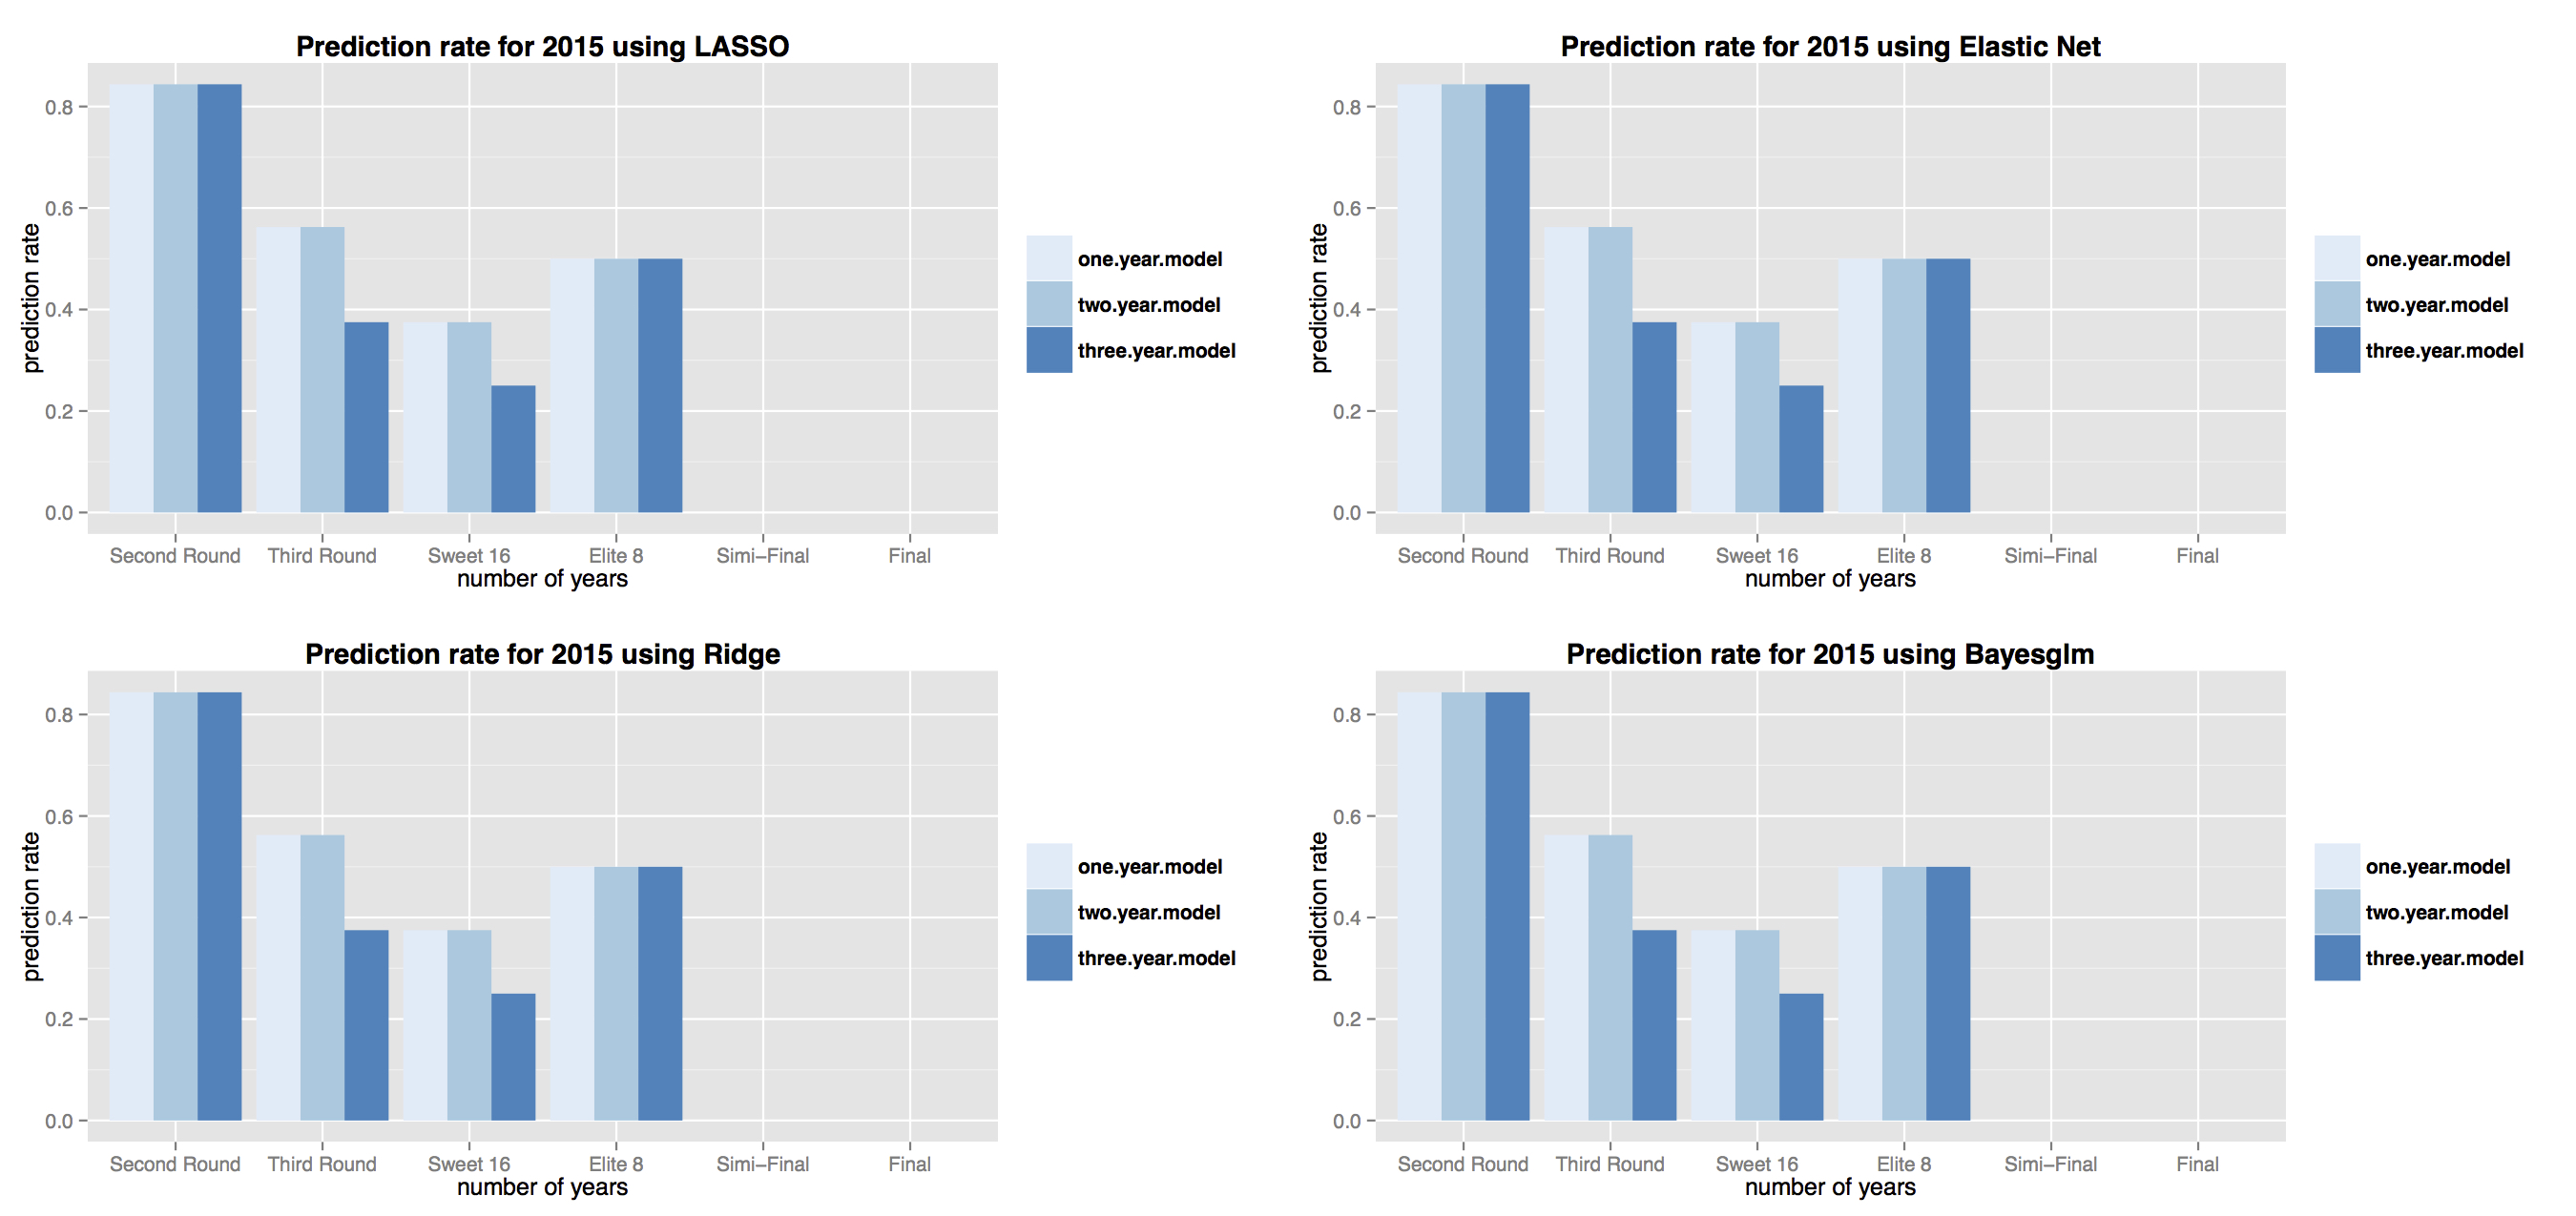
\includegraphics[scale = 0.17]{year.jpg}
\end{center}
\caption{2015 prediction rate for each round by models trained with 1-3 past year season data}

\begin{center}
   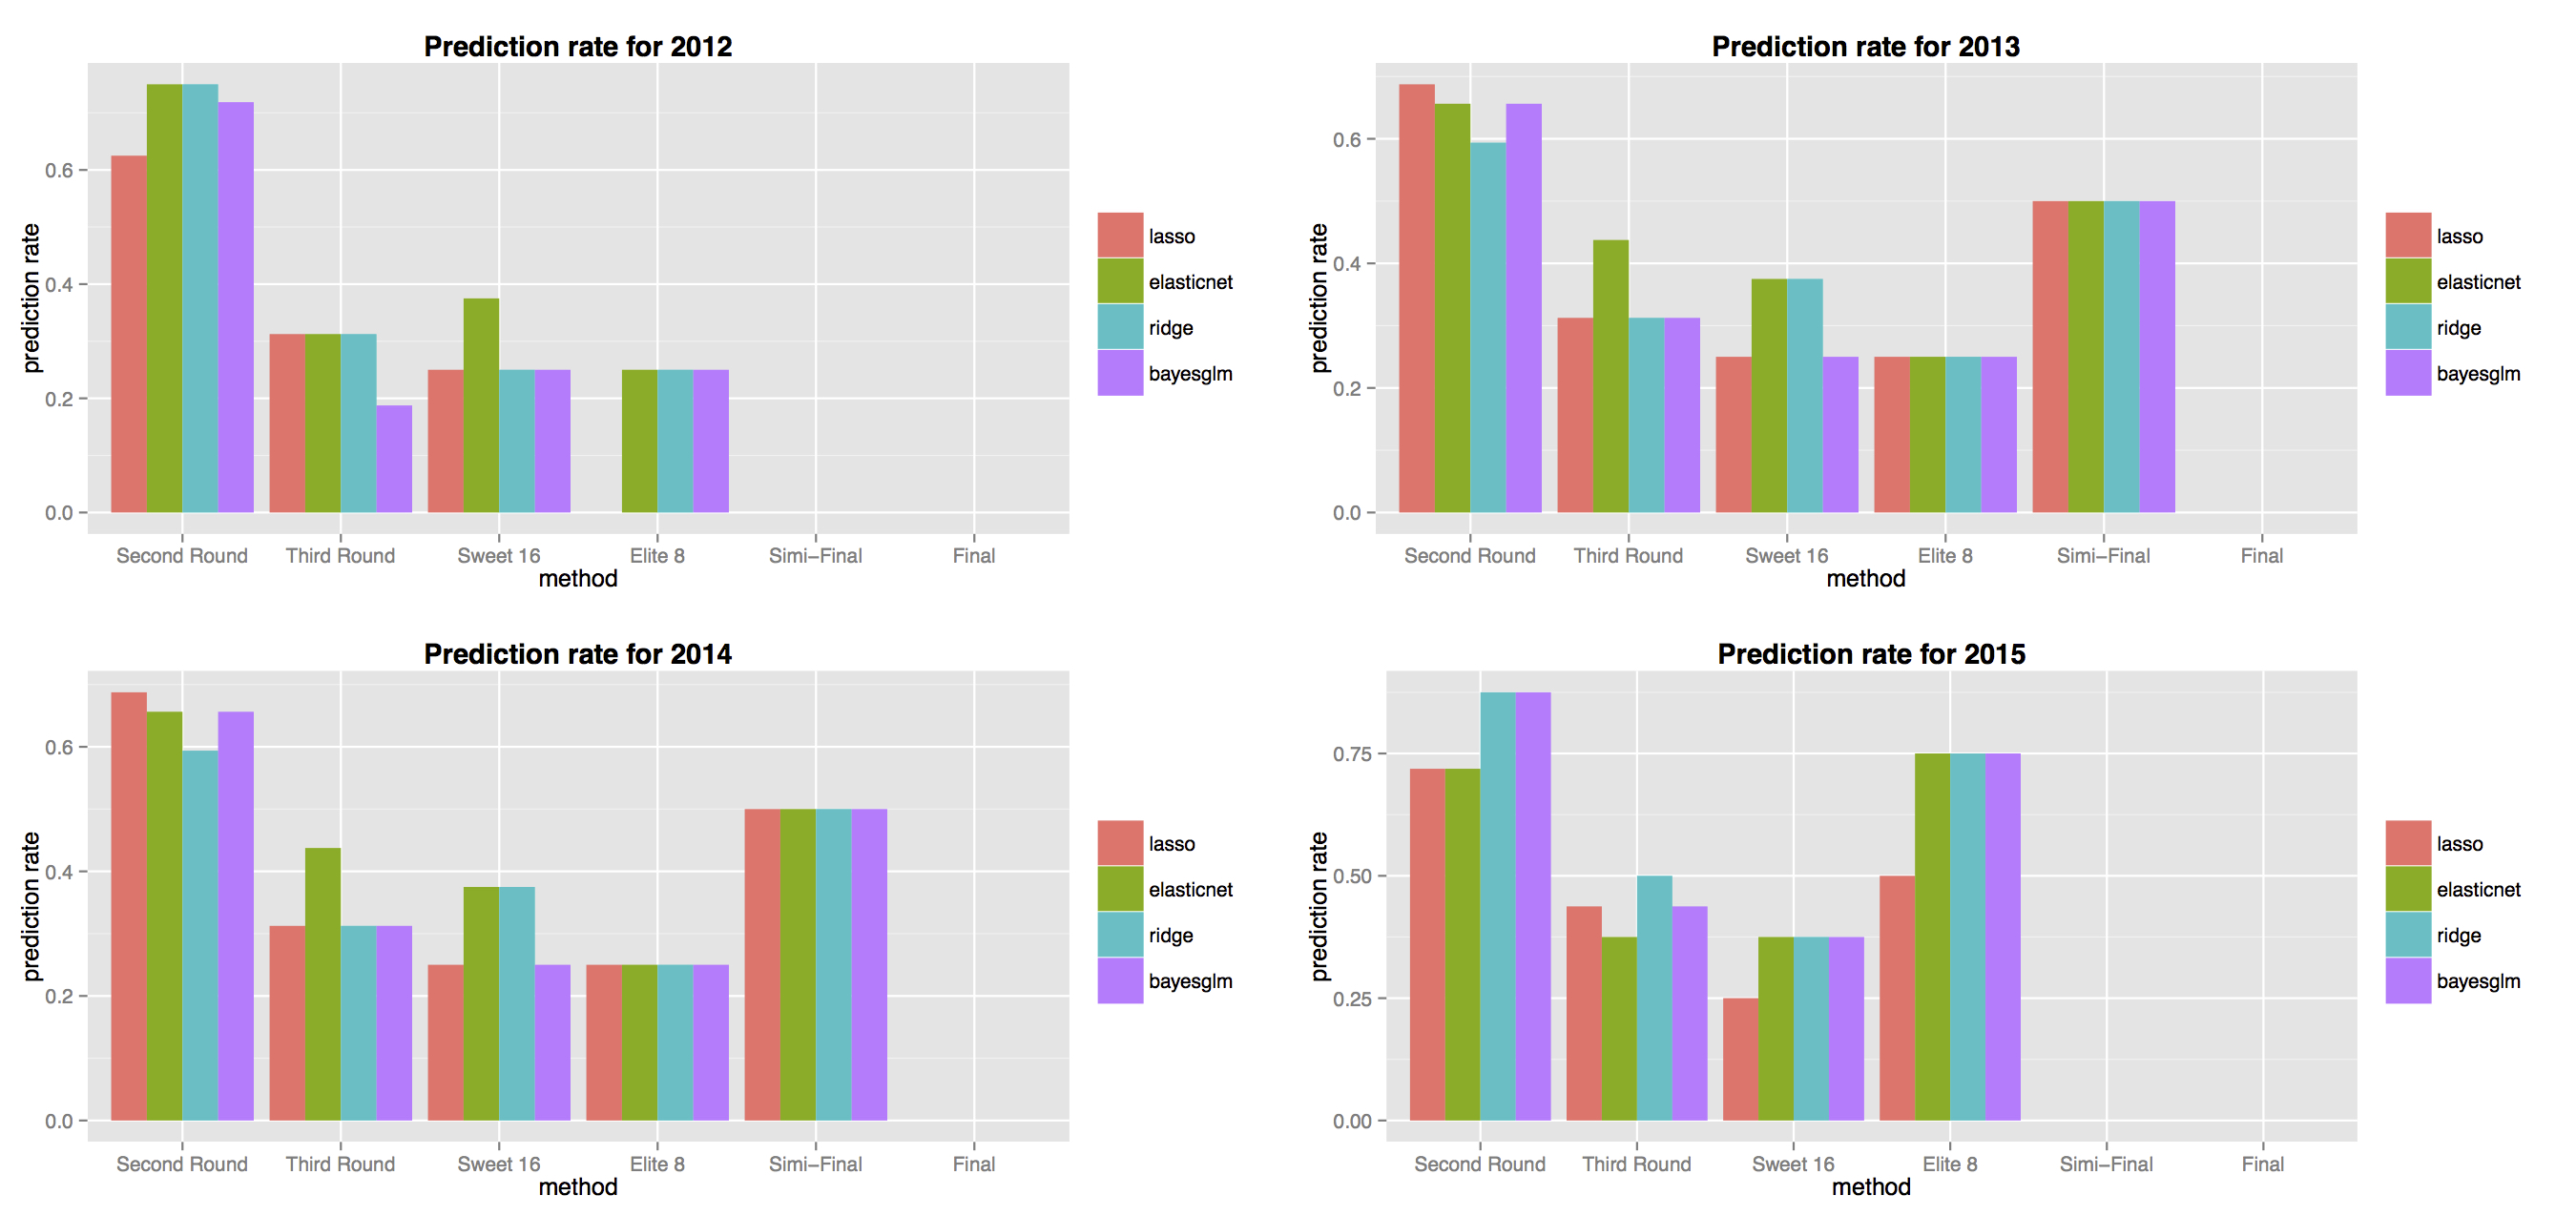
\includegraphics[scale = 0.17]{model.jpg}
\end{center}
\caption{Prediction rate from 2012 to 2015 predicted by each of our models}
\end{figure}

\begin{figure}[H]
\begin{center}
   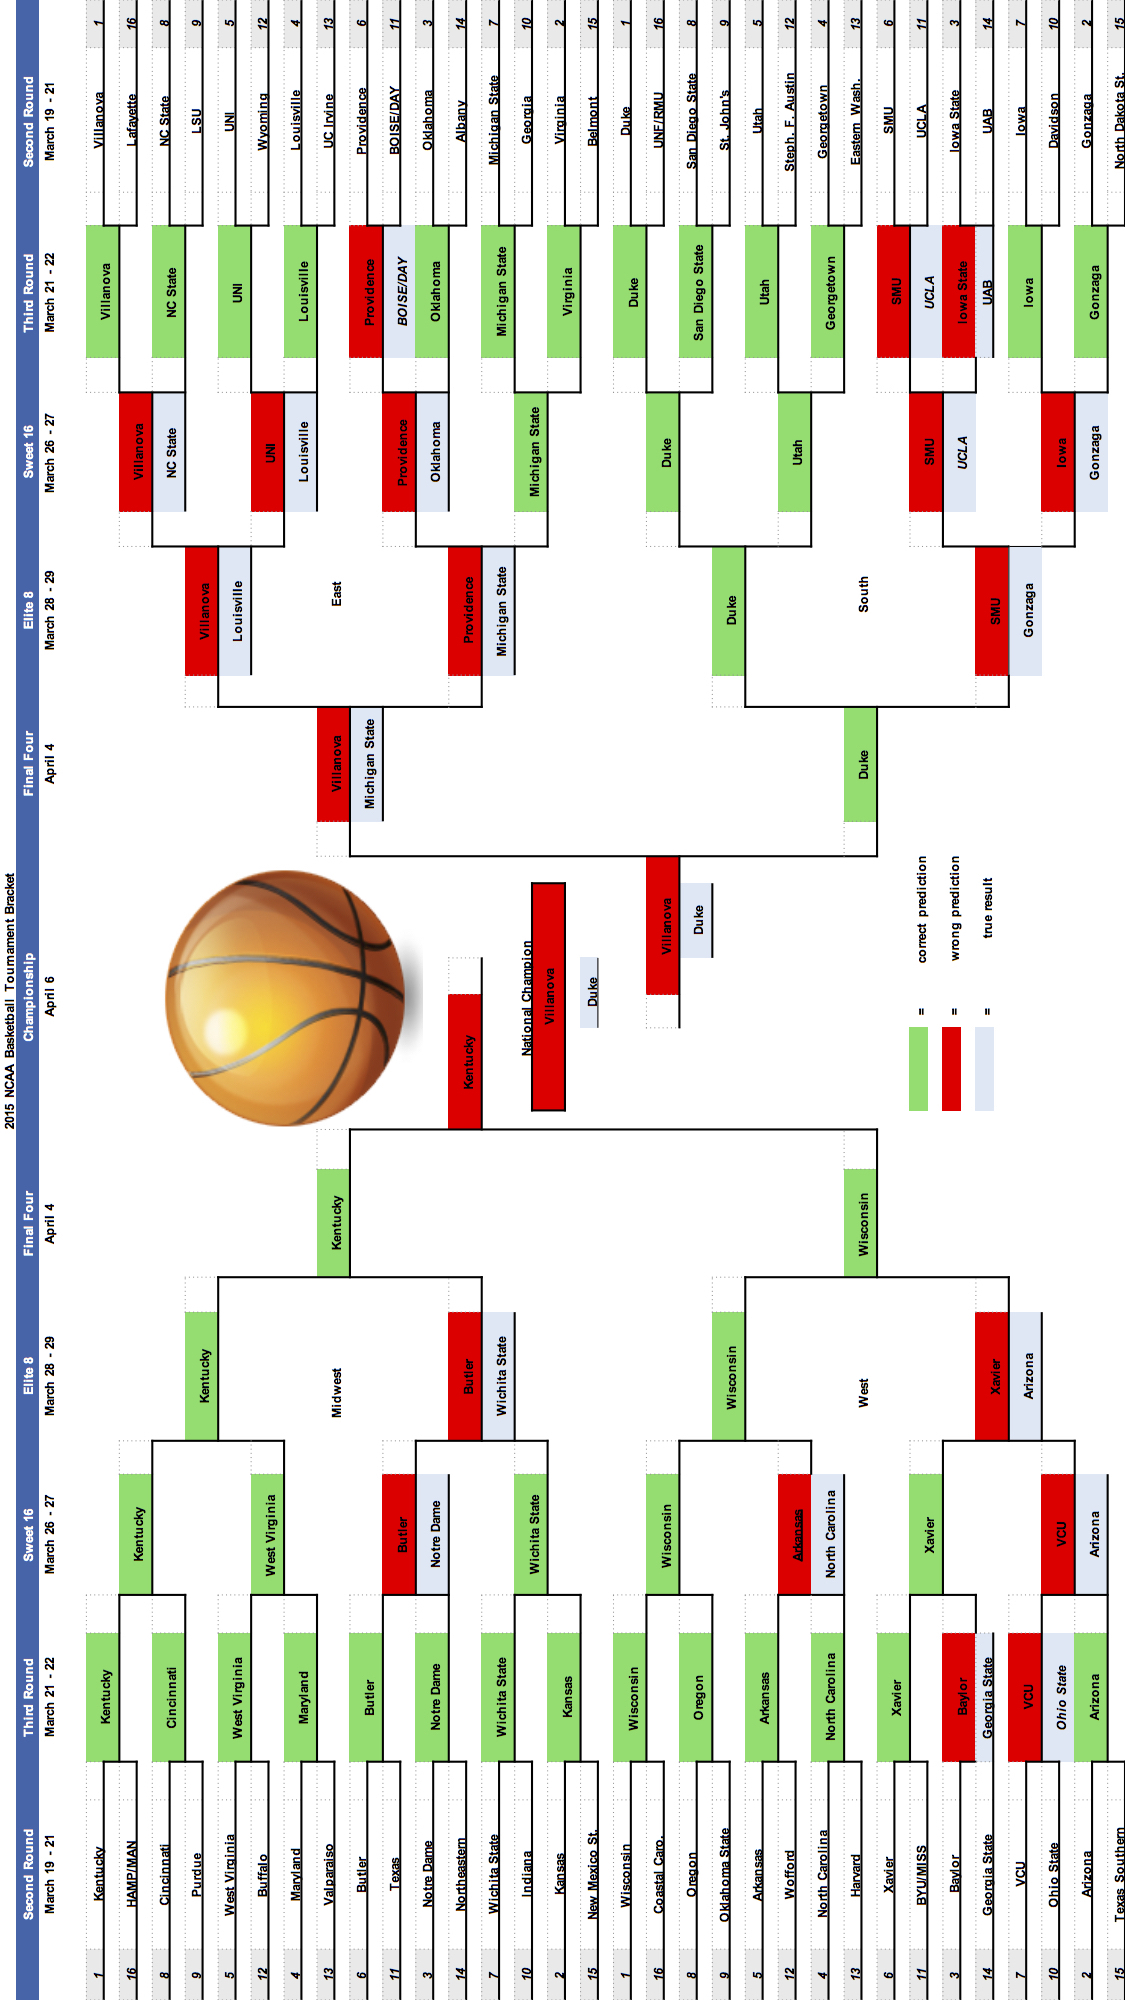
\includegraphics[scale = 0.3]{bracket.jpg}

\caption{Ridge regression prediction bracket for 2015}
\end{center}
\end{figure}





\end{document}